% \paragraph{}

% \begin{figure}[b!]
% 	\capstart
% 	\centering
% 	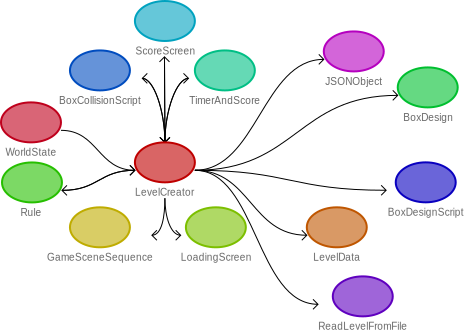
\includegraphics[width=0.7\textwidth]{images/LevelCreator_class_connectivity}
% 	\caption[LevelCreator class chart]{This is how we have connected classes to LevelCreator.}
% 	\label{fig:LevelCreator_chart}
% \end{figure}


Since we have aimed for making an environment, we have built cogARC around 
the concept of making new levels. Because of this the most important module 
is the LevelCreator. As we see from \autoref{fig:LevelCreator_chart}, there
are quite many classes that LevelCreator uses.

\begin{wrapfigure}{r}{0.6\textwidth}
	\capstart
	\centering
	\vspace{-5pt}
	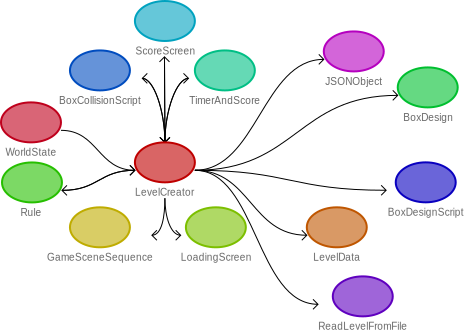
\includegraphics[width=0.58\textwidth]{images/LevelCreator_class_connectivity}
	\caption[LevelCreator class chart]{This is how we have connected classes to LevelCreator.}
	\label{fig:LevelCreator_chart}
	\vspace{-10pt}
\end{wrapfigure}

The arrows indicate that the class use some functionality or data in the 
class that is pointed to. This means that all the other classes are used by
LevelCreator and some classes use LevelCreator. An example of the latter is 
WorldState that set up the state of the game according to what it finds in the
LevelCreator.

LevelData is also quite important for the creator. As it's name says, the data
for the level are stored here.



% \todo{Charts of how objects are connected.}

% \begin{figure}[h!]
%         \capstart
%         \centering
%         \includegraphics[width=0.68\textwidth]{images/game_world_class_chart}
%         \caption[World game class chart]{Simplified, this is how the game world is connected.}
%         \label{fig:world_game}
% \end{figure}

\paragraph{}

\autoref{fig:world_game} shows a simplified chart of how cogARC is connected.
To explain this we can start with WorldState. The state of the world depends on
how the LevelCreator are set up. It will also be affected by which rules that
are currently used. 
The rule script interferes with GameSceneSequence to load the proper level,
i.e. when a level have been cleared. The LevelCreator use BoxDesignScript to
load the proper design on the cubes.

\begin{wrapfigure}{l}{0.5\textwidth}
        \capstart
        \centering
        \includegraphics[width=0.48\textwidth]{images/game_world_class_chart}
        \caption[World game class chart]{Simplified, this is how the game world is connected.}
        \label{fig:world_game}
        \vspace{-10pt}
\end{wrapfigure}

Both the LevelCreator and the Rule script needs to know whether a box have
collided or not, hence they need BoxCollisionScript. To discern when a collision
happens, the BoxCollisionScript will need to know where the object are placed
in the world. The GyroRotor use the embedded gyro sensor in the gaming device
to give an answer to this. The TransformDistributor is also important for 
BoxCollisionScript. It will tell the ID of the markers, so that it is possible
to see which objects that actually collided. When the Rule script figures out
that a solution is found upon a box collision event, the WorldState will be
updated and the testing object will be destroyed by a triggering of
SelfdestructObject. This will end the collision testing of the given box, but 
the box itself will still be visible on the screen.

With this structure the state of the gameworld will be continuously updated
and different scripts will do different tasks.

